\documentclass[12pt]{beamer}
%\mode<presentation>{\usetheme{Copenhagen}}
\mode<presentation>{\usetheme{JuanLesPins}}
\usecolortheme{default}
%\usecolortheme{beetle}
\useoutertheme{} % Define el encabezado y pie de página. Puedes elegir entre: {infolines}, {miniframes}, {shadow}, {sidebar}, {smoothbars}, {smoothtree}, {split}, {tree}...
\useinnertheme{circles} %  Define el formato de los puntos. Puedes elegir entre: {circles}, {inmargin}, {rectangles}, {rouded}...
%\usepackage[spanish, es-tabla]{babel}
\usepackage[utf8]{inputenc} % ansinew para windows, latin1 para unix
\usepackage{amssymb}
\usepackage{amsfonts}
\usepackage{amsthm}
\usepackage{mathrsfs}
\usepackage{listings}
\usepackage{multirow}
% % %\usepackage{dsfont}
\usepackage{amsmath}
\usepackage{amscd}
\usepackage{graphicx}
\usepackage{mathtools}
% % %\usepackage[all,cmtip]{xy}
\usepackage{fancyhdr}
\usepackage{geometry}
\usepackage{graphicx}
\usepackage{setspace}
\usepackage{subfigure}
\usepackage{multicol}
\usepackage{tikz}



\title{The News Classifier}
\subtitle{ Final Project  }
\titlegraphic{
\includegraphics[width=2cm]{ironhack_logo.png}} 
\author{Ulises Aquino \\ and Javier Alvarez Jiménez}

%\titlegraphic{%
%  \begin{picture}(0,0)
%    \put(30,-20){\makebox(0,0)[rt]{
\includegraphics[width=2cm]{ironhack_logo.png}}}
 % \end{picture}}



%\institute[IH]{IronHack \\
%Mexico\\[\medskipamount]
%      
\includegraphics[width=\textwidth,height=.9 \textheight]{ironhack_logo.png}}
 
\institute[IH]{IronHack \\
Mexico }
 
\date{December 2019} 
      
    
%\and
%Seminario de Gravitación y Cosmología, \\
%UAM.


\begin{document}
\frame{\titlepage}


%\begin{frame}%[allowframebreaks]

%\frametitle{Índice}

%\tableofcontents
%\tableofcontents

%\end{frame}
\section{Introduction}

\begin{frame}

\frametitle{The News}
\begin{figure}  \label{fig:papers}
  %\centering
  
	\begin{itemize}
	\item Nowadays, we have a lot of information, news included.
	\end{itemize}  
  
   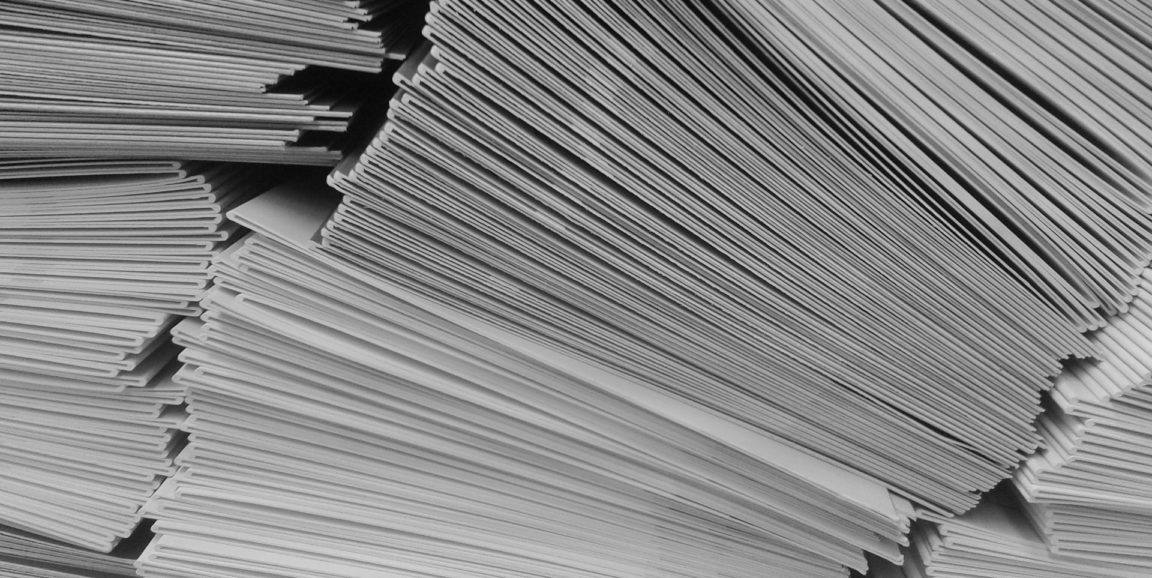
\includegraphics[width=0.3\textwidth]{muchpaper.jpg}
  %\caption{$I_{\alpha \alpha}$ para calcular la componente $G_{\alpha \alpha}$ del TGC.}
  \label{fig:papers}
\end{figure}

\begin{figure}  \label{fig:bias}
  %\centering
  
	\begin{itemize}
	\item The information can be biased.
	\end{itemize}  
  
   
\includegraphics[width=0.3\textwidth]{bias.png}
  %\caption{$I_{\alpha \alpha}$ para calcular la componente $G_{\alpha \alpha}$ del TGC.}
  \label{fig:bias}
\end{figure}





\end{frame}
\begin{frame}
\frametitle{Steps}
\begin{itemize}
\item We scrap as many news as we can
\item We make a sentiment analysis for all the news (SentimentIntensityAnalyzer from nltk)
\item We clusterize the news (vectorization with TfidfVectorizer, clustering with HDBSCAN and cosine similarity)
\item We summarize every cluster, and get a sentiment score per cluster
\item We upload all the work to mongodb (harder than it sound, ids, structure, etc)
\end{itemize}
\end{frame}

\begin{frame}
\frametitle{Text Summarization\footnote[frame]{https://stackabuse.com/text-summarization-with-nltk-in-python/} } 
Algorithm:
\begin{itemize}
\item Text $\rightarrow $ sentences
\item Get bag of words (avoid stop words, cleaning)
\item Give scores to words (in this case, according to the relative frequency)
\item From words scores, we can rate the sentences
\item We keep the sentences with the highest scores
\end{itemize}


\end{frame}
\section{Future Steps}
\begin{frame}
\frametitle{Recommendation System}
We want to build a recommendation System for the article.
We use look for the most similar user and recommend articles from it.
The key point is to get scores from the users.
\begin{itemize}
\item $+1$ if the user read the article
\item $+1$ if the user saves the article
\item If the user comments the article, we make a sentiment analysis  and we add the compound value
\end{itemize}
\end{frame}
\begin{frame}
\frametitle{Improvements}

 The clustering system
 \begin{figure}  \label{fig:good}
  %\centering
  
  
   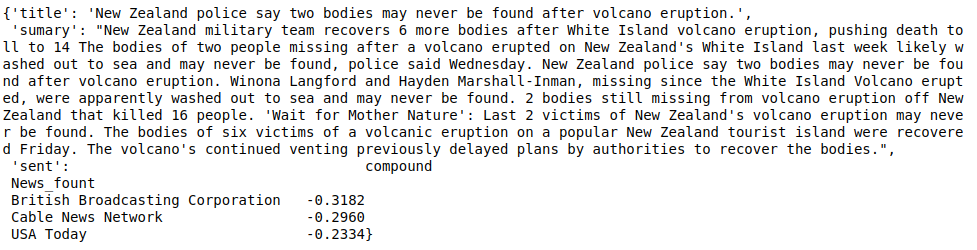
\includegraphics[width=1  \textwidth]{good.png}
  \caption{Good cluster.}
  \label{fig:good}
\end{figure}



\begin{figure}  \label{fig:bad}
  %\centering
  
  
   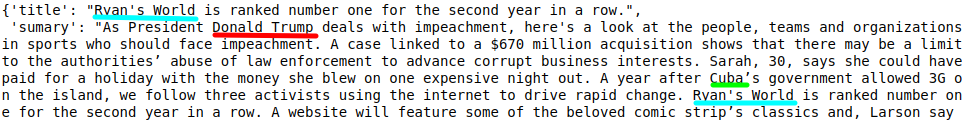
\includegraphics[width=1\textwidth]{bad.png}
  \caption{Bad cluster.}
  \label{fig:bad}
\end{figure}
\end{frame}



\begin{frame}
\begin{itemize}
\item Ideas after use it
\item Suggestions...
\end{itemize}
\end{frame}
\end{document}

\subsection{Tensor Geométrico Cuántico}
\begin{frame} 
\frametitle{Tensor Geométrico Cuántico}Supongamos que el sistema depende de $L$ parámetros $\lambda^\alpha$, $\alpha=1,...,L$ y consideremos $ \left\vert \psi' \right> = \left\vert \psi(\lambda+\delta\lambda) \right>$, entonces
\begin{equation}
\left\vert \psi(\lambda + \delta \lambda) \right> = 1 + \left\vert \psi(\lambda) \right> + \left\vert \partial_\alpha \psi(\lambda) \right> \delta \lambda^\alpha + \frac{1}{2} \left\vert \partial_\alpha \partial_\beta \psi(\lambda) \right> \delta \lambda^\alpha \delta \lambda^\beta + ...
\end{equation}
y
\begin{align} \label{eq:traslsegor}
\left< \psi(\lambda) \right. \left\vert \psi(\lambda + \delta \lambda) \right> = 1 + \left<  \psi(\lambda) \right. \left\vert \partial_\alpha \psi(\lambda) \right> \delta\lambda^\alpha \nonumber \\ + \frac{1}{2} \left< \partial\psi(\lambda) \right. \left\vert \partial_\alpha \partial_\beta \psi(\lambda) \right> \delta \lambda^\alpha \delta \lambda^\beta +...
\end{align}
\end{frame}
\begin{frame}
Tomando la norma al cuadrado de  (\ref{eq:traslsegor}), se obtiene
\begin{equation}
| \left< \psi(\lambda) \right. \left\vert \psi(\lambda + \delta \lambda) \right> |^2 = F^2(\lambda,\lambda+\delta\lambda)= 1- G_{\alpha \beta}\delta \lambda^\alpha \delta \lambda^\beta+...
\end{equation}
donde
%\begin{alertblock}{Tensor Geométrico Cuántico}
\begin{equation}
G_{\alpha \beta} =  \left< \partial_\alpha \psi | \partial_\beta \psi \right> - \left<\partial_\alpha \psi | \psi \right> \left< \psi | \partial_\beta \psi \right>
\end{equation}
%\end{alertblock}
es el tensor geométrico cuántico. 
\end{frame}

\begin{frame}
Claramente sólo la parte simétrica de 
 $G_{\alpha \beta}$ es importante en el desarrollo en serie de la Fidelidad. \\
El tensor métrico de información cuántica es
\begin{equation}
g_{\alpha \beta} = \textbf{Re} G_{\alpha \beta} = \frac{1}{2} \left( \left< \partial_\alpha \psi | \partial_\beta \psi \right> + \left< \partial_\beta \psi | \partial_\alpha \psi \right> \right) - \left<\partial_\alpha \psi | \psi \right> \left< \psi | \partial_\beta \psi \right>. 
\end{equation}
La parte antisimétrica también tiene un significado físico. Si tomamos
\begin{equation}
A_\alpha = i \left< \psi \right| \left. \partial_\alpha \psi \right>,
\end{equation}
\end{frame}
\begin{frame}


se puede definir 
\begin{equation}
F_{\alpha \beta} = \frac{\partial A_\alpha}{\partial \lambda^\beta} - \frac{\partial A_\beta}{\partial \lambda^\alpha},
\end{equation}
el cual corresponde a la parte imaginaria del Tensor Geométrico Cuántico
\begin{equation}
\frac{1}{2} F_{\alpha \beta} = \textbf{Im} G_{\alpha \beta} = \frac{1}{2i}\left( \left< \partial_\alpha  \psi | \partial_\beta \psi \right> - \left< \partial_\beta \psi | \partial_\alpha \psi \right> \right),
\end{equation}
y corresponde con la curvatura de Berry.
\end{frame}
%\section{Cambio de norma generalizado.}



%\subsection{Cambio de Norma}
\begin{frame}
\frametitle{Cambio de Norma}
Si agregamos una fase que sólo depende de los parámetros
\begin{equation}
\psi_\alpha = e^{i \alpha(\lambda)}\psi,
\end{equation}
\begin{equation}
\left< \psi_\alpha(\lambda) | \psi_\alpha(\lambda') \right> = e^{i(\alpha-\alpha')}\left< \psi(\lambda) | \psi(\lambda') \right> ,
\end{equation}
Como sólo es una fase
\begin{equation}
F(\psi_\alpha(\lambda), \psi_\alpha(\lambda')) = F(\psi(\lambda), \psi(\lambda')),
\end{equation}
similarmente
\begin{equation}
g'_{ij} = g_{ij}.
\end{equation}
\end{frame}
\begin{frame}
En cambio, cuando 
\begin{equation}
\alpha = \alpha( \lambda, x,p)
\end{equation} 
\begin{equation}
F(\psi_\alpha(\lambda), \psi_\alpha(\lambda')) \neq F(\psi(\lambda), \psi(\lambda')),
\end{equation}
similarmente
\begin{equation}
g'_{ij} \neq g_{ij}.
\end{equation}
Este resultado fue publicado en JMP.
\end{frame}

\section{Perspectiva Lagrangiana}
\subsection{Tensor Geométrico Cuántico}
%\begin{frame}
%\frametitle{Perspectiva Lagrangiana}
%Tenemos varias formas para calcular el Tensor Geométrico Cuántico
%\begin{equation}
%G_{\alpha \beta} =  \left< \partial_\alpha \psi | \partial_\beta \psi \right> - \left<\partial_\alpha \psi | \psi \right> \left< \psi | \partial_\beta \psi \right>,
%\end{equation}
%\begin{equation}
%F(\lambda,\lambda+\delta\lambda)=1-\dfrac{1}{2}G_{\alpha \beta}\delta\lambda^\alpha \delta \lambda^\beta,
%\end{equation}
%\begin{equation}
%G_{\alpha \beta}= \sum_{n \neq 0} \frac{\left<\psi_0 \right\vert \partial_\alpha H \left\vert \psi_n \right> \left<\psi_n \right\vert \partial_\beta H \left\vert \psi_0 \right>}{\left(E_0-E_n \right)^2},
%\end{equation}
%sin embargo, nos gustaría una expresión que use la integral de trayectoria para hacer más fácil la aplicación en teoría cuántica de campos.
%\end{frame}

\begin{frame}
\frametitle{Tensor Geométrico Cuántico desde una perspectiva Lagrangiana}
Hasta ahora, todos los cálculos se han hecho utilizando la función de onda.
\begin{equation}
G_{\alpha \beta} =  \left< \partial_\alpha \psi | \partial_\beta \psi \right> - \left<\partial_\alpha \psi | \psi \right> \left< \psi | \partial_\beta \psi \right>.
\end{equation}
\\ 
 Para evitar esto, usaremos el formalismo de integral de trayectoria.
 

\end{frame}






\begin{frame}
 Consideremos una teoría descrita por el lagrangiano $\mathcal{L}_0$ para $t_0=(-\infty,0)$  y $\mathcal{L}_1=\mathcal{L}_0 +  \mathcal{O}_\alpha \delta \lambda^\alpha$ para $t=(0,\infty)$, entonces
\begin{eqnarray}
\left< q_1,t | q_0, t_0 \right> = \sum_{n_0,n_1} \left< q_1, t | n_1\right> \left< n_1 | n_0 \right> \left< n_0 | q_0, t_0 \right> \nonumber \\ = \sum_{n_0,n_1} \left< q_1\right| e^{- i t E(n_1)} \left| n_1\right> \left< n_1 | n_0 \right> \left< n_0 \right| e^{it_0 E(n_0)} \left| q_0 \right>,
\end{eqnarray}
Los subíndices  $1$ y $0$ indican qué lagrangiano describe la teoría
\end{frame}
\end{document}
\begin{frame}
Haciendo una rotación de Wick y tomando los límites
\begin{equation}
t \longrightarrow -i \tau,
\end{equation}
\begin{equation}
\tau \longrightarrow \infty,  \ \ \ \tau_0 \longrightarrow - \infty,
\end{equation}
los términos dominantes serán los del edo. base.
\begin{eqnarray}
\left< q_1,\infty | q_0,-\infty \right> &=& e^{- \tau E(0_1)} e^{\tau_0E(0_0)}  \left< q_1 | 0_1\right> \left< 0_1 | 0_0 \right> \left< 0_0 | q_0 \right> \nonumber \\ &=& \left< q_1,\infty | 0_1\right> \left< 0_1 | 0_0 \right> \left< 0_0 | q_0, -\infty \right>. \end{eqnarray}
Notemos que los vacíos son diferentes en $\pm \infty$. Despejando
\begin{equation} \label{eq:traspsants}
\left< 0_1 | 0_0 \right> = \dfrac{\left< q_1,\infty | q_0,-\infty \right>}{\left< q_1,\infty | 0_1 \right> \left< 0_0 | q_0,-\infty \right>}.
\end{equation}
\end{frame}

\begin{frame} 
Trataremos de reescribir todo en términos de integral de trayectoria. En el primer término 
\small
\begin{eqnarray} \label{eq:trasidcamc}
&&\left<  q_1, \infty| q_0,-\infty \right> = \int dq \left< q_1,\infty | q, t=0 \right> \left< q, t=0 | q_0,-\infty \right>\nonumber \\
&=& \int dq \int_{q(t=0)}^{q(\infty)} \mathcal{D}q e^{- \int_0^\infty d\tau' \mathcal{L}_1} \int_{q(-\infty)}^{q(t=0)} \mathcal{D} q e^{-  \int_{-\infty}^0 d\tau' \mathcal{L}_0}, \nonumber \\ &=& \int_{q(-\infty)}^{q(\infty)} \mathcal{D}q \exp\left(-\int_{-\infty}^0d\tau  \mathcal{L}_0 - \int_0^\infty d\tau (\mathcal{L}_0 + \delta \lambda^\alpha \mathcal{O}_\alpha)\right) \nonumber \\  &=& \int_{q(-\infty)}^{q(\infty)} \mathcal{D}q \exp\left(-\int_{-\infty}^\infty d\tau  \mathcal{L}_0 - \int_0^\infty d\tau  \delta \lambda^\alpha \mathcal{O}_\alpha\right)
\end{eqnarray}
\normalsize
\end{frame}
\begin{frame}
ahora notamos que
\begin{equation}
Z_i = \int \mathcal{D} q \exp\left(- \int_{-\infty}^\infty d\tau  \mathcal{L}_i \right),
\end{equation}
y pidiendo simetría ante inversión temporal, interpretamos
\begin{equation}
\left< q_1,\tau | 0_1 \right> = \sqrt{Z_1},
\end{equation} 
\begin{equation}
\left< 0_0 | q_0,\tau_0 \right> = \sqrt{Z_0},
\end{equation}
\end{frame}
\begin{frame}
En estas condiciones, la ecuación (\ref{eq:traspsants}) se puede escribir como
\begin{eqnarray} \label{eq:trasinttra}
\left< 0_1 | 0_0 \right> =   \dfrac{\int \mathcal{D} q \left( e^{ -\int_{-\infty}^\infty d\tau  \mathcal{L}_0 } e^{-\int_{0}^\infty d\tau   \delta\lambda^\alpha \mathcal{O}_\alpha }\right)}{\sqrt{Z_0 Z_1}}.
\end{eqnarray} 
Pero recordando que
\begin{equation}
\left< A \right> = \frac{1}{Z_0} \int \mathcal{D} q \left[ \exp \left( - \int_{-\infty}^\infty d\tau  \mathcal{L}_0\right) A(q) \right],
\end{equation}
es el promedio con respecto del sistema descrito por $\mathcal{L}_0$
\end{frame}
\begin{frame}
\begin{equation}
\left< 0_1 | 0_0 \right>=\frac{\left< e^{-\int_0^\infty d\tau  \delta \lambda^\alpha \mathcal{O}_\alpha}\right>}{\sqrt{\frac{Z_1}{Z_0}}} = \frac{\left< e^{-\int_0^\infty d\tau  \delta \lambda^\alpha \mathcal{O}_\alpha}\right>}{\sqrt{\frac{\int \mathcal{D} q e^{-  \int_{-\infty}^\infty d\tau (\mathcal{L}_0 + \delta \lambda^\alpha \mathcal{O}_\alpha)}}{Z_0}}},
\end{equation}
 por tanto
\begin{equation} \label{eq:trasindtra}
\left< 0_1 | 0_0 \right> = \dfrac{\left< \exp\left( - \int_0^\infty d\tau  \delta\lambda^\alpha \mathcal{O}_\alpha(\tau)\right) \right>}{\sqrt{\left< \exp \left(- \int_{-\infty}^\infty d \tau  \delta \lambda^\alpha \mathcal{O}_\alpha(\tau) \right) \right>}}.
\end{equation}
\end{frame}
\begin{frame}

\begin{equation}
\left| \left< 0_1\right| \left. 0_0 \right>\right|^2= \dfrac{\left< e^{\left(- \int_{0}^\infty d \tau  \delta \lambda^\alpha \mathcal{O}_\alpha(\tau) \right)} \right> \left<  e^{\left( -\int_{- \infty}^0 d \tau  \delta \lambda^\alpha \mathcal{O}_\alpha(\tau) \right)} \right>}{\left< \exp \left(- \int_{- \infty}^\infty d \tau  \delta \lambda^\alpha \mathcal{O}_\alpha(\tau) \right) \right>},
\end{equation}

la serie da
\small
\begin{eqnarray}
&\left| \left< 0_1 | 0_0 \right>\right|^2 =  1 \nonumber \\ &-  \int_{-\infty}^0 d\tau_1 \int_{0}^\infty d \tau_2  \left[ \left< \mathcal{O}_\alpha(\tau_1) \mathcal{O}_\beta (\tau_2) \right>  \right.  \left. - \left< \mathcal{O}_\alpha(\tau_1) \right> \left< \mathcal{O}_\beta (\tau_2) \right> \right]\delta \lambda^\alpha \delta \lambda^\beta. \nonumber \\
\end{eqnarray}

\end{frame}
\begin{frame}
pero
\
\begin{equation}
\left| \left< 0_1 | 0_0 \right>\right|^2 = F^2(0_0, 0_1) = 1  -  G_{\alpha \beta}\delta \lambda^\alpha  \delta \lambda^\beta,
\end{equation}
entonces \\
\small
\begin{align}\label{eq:tgcdc}
G_{\alpha \beta}  =   \int_{-\infty}^0 d\tau_1 \int_0^{\infty} d \tau_2 \left[  \left< \mathcal{O}_\alpha(\tau_1) \mathcal{O}_\beta(\tau_2)\right> \right.  \left. - \left< \mathcal{O}_\alpha(\tau_1) \right> \left< \mathcal{O}_\beta(\tau_2)\right> \right].
\end{align}
\normalsize
\end{frame}
\begin{frame}
La parte real es
\small
\begin{eqnarray} \label{eq:tmqintdetra}
 \textbf{Re} G_{\alpha \beta}  =   \textbf{Re} \int_{-\infty}^0 d\tau_1 \int_0^{\infty} d \tau_2 \left[  \left< \mathcal{O}_\alpha(\tau_1) \mathcal{O}_\beta(\tau_2)\right> \right.  \left. - \left< \mathcal{O}_\alpha(\tau_1) \right> \left< \mathcal{O}_\beta(\tau_2)\right> \right] \nonumber \\ =  \int_{-\infty}^0 d\tau_1 \int_0^{\infty} d \tau_2 \left[ \frac{1}{2} \left( \left< \mathcal{O}_\alpha(\tau_1) \mathcal{O}_\beta(\tau_2)\right> + \left< \mathcal{O}_\alpha(\tau_1) \mathcal{O}_\beta(\tau_2)\right> \right) \right. \nonumber \\  \left. - \left< \mathcal{O}_\alpha(\tau_1) \right> \left< \mathcal{O}_\beta(\tau_2)\right> \right] \nonumber \\  = \int_{-\infty}^0 d\tau_1 \int_0^{\infty} d \tau_2 \left[ \frac{1}{2} \left< \left\lbrace \mathcal{O}_\alpha(\tau_1), \mathcal{O}_\beta(\tau_2) \right\rbrace \right> \right.  \left. - \left< \mathcal{O}_\alpha(\tau_1) \right> \left< \mathcal{O}_\beta(\tau_2)\right> \right] \nonumber 
\end{eqnarray} 
\end{frame}
\begin{frame}
y la parte imaginaria es
\small
\begin{eqnarray}
\textbf{Im} G_{\alpha \beta} &=& \frac{1}{2 i}  \int_{-\infty}^0 d\tau_1 \int_0^{\infty} d \tau_2  \left(  \left< \mathcal{O}_\alpha(\tau_1) \mathcal{O}_\beta(\tau_2)\right> -   \left< \mathcal{O}_\alpha(\tau_1) \mathcal{O}_\beta(\tau_2)\right>  \right) \nonumber \\
\end{eqnarray}
\normalsize
\begin{equation}
 \ \ = \frac{1}{2 i}  \int_{-\infty}^0 d\tau_1 \int_0^{\infty} d \tau_2  \left< \left[ \mathcal{O}_\alpha(\tau_1), \mathcal{O}_\beta(\tau_2) \right]\right>. 
\end{equation}
\end{frame}
\begin{frame}
por lo tanto
\small
\begin{equation} \label{eq:tmcdc}
g_{\alpha \beta} = \int_{-\infty}^0 d\tau_1 \int_0^{\infty} d \tau_2 \left[ \frac{1}{2} \left< \left\lbrace \mathcal{O}_\alpha(\tau_1), \mathcal{O}_\beta(\tau_2) \right\rbrace \right> - \left< \mathcal{O}_\alpha(\tau_1) \right> \left< \mathcal{O}_\beta(\tau_2)\right> \right]
\end{equation}
\normalsize
\  y
\begin{equation} \label{eq:cbdc}
F_{\alpha \beta} =  \frac{1}{ i}  \int_{-\infty}^0 d\tau_1 \int_0^{\infty} d \tau_2  \left< \left[ \mathcal{O}_\alpha(\tau_1), \mathcal{O}_\beta(\tau_2) \right]\right>. 
\end{equation}
Estas expresiones están  en términos de funciones de correlación a tiempos distintos.
\end{frame}
\begin{frame}
Podemos traducir a teoría cuántica de campos. El tensor métrico toma la forma
\begin{eqnarray}
g_{\alpha \beta}  =   \int_{-\infty}^0 d\tau_1 \int_0^{\infty} d \tau_2 \int dx_1 dx_2 \left[ \frac{1}{2} \left< \left\lbrace \mathcal{O}_\alpha(\tau_1, \vec{x}_1), \mathcal{O}_\beta(\tau_2, \vec{x}_2) \right\rbrace \right> \right. \nonumber \\ \left. - \left< \mathcal{O}_\alpha(\tau_1, \vec{x}_1) \right> \left< \mathcal{O}_\beta(\tau_2, \vec{x}_2)\right> \right],
\end{eqnarray}
mientras que la curvatura de Berry se transforma en
\begin{equation} 
F_{\alpha \beta} =  \frac{1}{i} \int_{-\infty}^0 d\tau_1 \int_0^{\infty} d \tau_2 \int dx_1 dx_2   \left< \left[ \mathcal{O}_\alpha(\tau_1,\vec{x}_1), \mathcal{O}_\beta(\tau_2, \vec{x}_2) \right] \right>.
\end{equation}

\end{frame}
\begin{frame}
\frametitle{Oscilador Armónico Generalizado}
El Hamiltoniano de este sistema es

\begin{equation} \label{eq:hamosgen}
H= Z p^2 + Y \left\lbrace p,q \right\rbrace + X q^2,
\end{equation}

los operadores están dados por
\begin{equation}
O_X = - q^2,
\end{equation}
\begin{equation}
O_Y = - \left\lbrace q,p \right\rbrace,
\end{equation}
\begin{equation}
O_Z = -p^2.
\end{equation}
\end{frame}
\begin{frame}
 hacemos la transformación canónica
\begin{equation} \label{eq:trancpc}
q=\sqrt{Z}Q,
\end{equation}
\begin{equation} \label{eq:trancpm}
p=\dfrac{1}{\sqrt{Z}}\left(P-YQ \right),
\end{equation}
con la que el Hamiltoniano toma la forma
\begin{equation}
H'= P^2 + \Omega^2 Q^2,
\end{equation}
donde $\Omega=\sqrt{XZ-Y^2}$. Por lo tanto
\begin{equation}
E_n = 2 \hbar \Omega \left( n+ 1/2\right),
\end{equation}
\end{frame}
\begin{frame}
y podemos escribir,
\begin{equation}
Q=\sqrt{\dfrac{\hbar}{2 \Omega}} \left(a^\dag+a \right),
\end{equation}
\begin{equation}
P=i \sqrt{\dfrac{\hbar \Omega}{2}} \left( a^\dag - a \right),
\end{equation}
donde $a$ y $a^\dag$ son operadores de aniquilación y creación usuales. Al tiempo $t$
\begin{equation}
a(t) = a e^{-2 i \Omega t},  \ \ \ a^\dagger(t) = a^\dagger e^{2 i \Omega t}.
\end{equation}
Con esto podemos calcular los valores esperados como si tuviéramos un oscilador usual.
\end{frame}
\begin{frame}
Primero notamos que
\begin{equation}
\left< O_X(t) \right> =- \dfrac{Z}{2 \Omega},
\end{equation}
\begin{equation}
\left< O_Y(t) \right> = \dfrac{Y}{ \Omega},
\end{equation} y 
\begin{equation}
\left< O_Z(t) \right> = -\dfrac{X}{2 \Omega},
\end{equation}
los cuales son independientes del tiempo.
\end{frame}
\begin{frame}
Para el término $g_{XY}$, encontramos que

\begin{equation}
\textbf{Re}\left< O_X(\tau_1) O_Y(\tau_2) \right> =  -\dfrac{YZ}{2 \Omega^2} - \dfrac{YZ}{\Omega^2} e^{-4 \Omega(\tau_1 - \tau_2)},
\end{equation}
y
\begin{equation}
\left< O_X(\tau_1) \right> \left<  O_Y(\tau_2) \right> = - \dfrac{YZ}{2 \Omega^2}.
\end{equation}
Por lo tanto 
\begin{equation}
g_{XY}= \int_{-\infty}^{0}d\tau_1  \int_{0}^{\infty}d\tau_2 \left[ -\dfrac{YZ}{2 \Omega^2} - \dfrac{YZ}{\Omega^2} e^{-4 \Omega(\tau_1 - \tau_2)} + \dfrac{YZ}{2 \Omega^2} \right].
\end{equation}
\end{frame}
\begin{frame}
Siguiendo el mismo procedimiento
\begin{eqnarray}
F_{ij}  = \dfrac{1}{16\left(XZ-Y^2 \right)^{3/2}}
\left(
\begin{array}{ccc}
0 & Z & -Y  \\
-Z & 0 & X \\
Y & -X & 0
\end{array}
\right),
\end{eqnarray}
\begin{eqnarray}
g_{ij}  = \dfrac{1}{32\left(XZ-Y^2 \right)^{2}}
\left(
\begin{array}{ccc}
Z^2 & - 2 ZY & 2 Y^2 - XZ  \\
- 2 ZY & 4 XZ & - 2 XY \\
2 Y^2 - XZ & - 2 XY & X^2
\end{array}
\right).
\end{eqnarray}
Los cálculos se pueden generalizar a sistemas de muchas partículas.  \\  Estos resultados fueron publicados en 
JHEP.
\end{frame}
\section{Tensor Geométrico Cuántico a partir de Funciones Generadoras}
\begin{frame}
\frametitle{Tensor Geométrico Cuántico a partir de Funciones Generadoras}
Consideremos al oscilador armónico con una perturbación del tipo $q^N$, 
\begin{equation}
H=\frac{1}{2}p^2 + \frac{\alpha}{2} q^2 + \lambda q^N,
\end{equation}
usaremos como parámetros $\lambda^1 = \alpha$ y $\lambda^2=\lambda$. Notemos que
\begin{equation}
H(\lambda^i+\delta \lambda^i) = H(\lambda^i) + \frac{\delta \alpha}{2}q^2 + \delta \lambda q^N,
\end{equation}
\end{frame}
\begin{frame}
por tanto
\begin{equation}
\mathcal{O}_\alpha = -\frac{q^2}{2}, \ \ \ \  \ \ \mathcal{O}_\lambda =- q^N,
\end{equation}

\begin{equation} \label{eq:QGTaaN}
G_{\alpha \alpha} = \frac{1}{4} \int_{-\infty}^0 d\tau_1 \int_0^\infty d\tau_2 \left[ \left< q^2(\tau_1) q^2(\tau_2) \right> - \left< q^2(\tau_1) \right> \left<q^2(\tau_2) \right> \right],
\end{equation}
\begin{equation}\label{eq:QGTalN}
G_{\alpha \lambda} = \frac{1}{2} \int_{-\infty}^0 d\tau_1 \int_0^\infty d\tau_2 \left[ \left< q^2(\tau_1) q^N(\tau_2) \right> - \left< q^2(\tau_1) \right> \left<q^N(\tau_2) \right> \right],
\end{equation}

\begin{equation}\label{eq:QGTllN}
G_{\lambda \lambda } =  \int_{-\infty}^0 d\tau_1 \int_0^\infty d\tau_2 \left[ \left< q^N(\tau_1) q^N(\tau_2) \right> - \left< q^N(\tau_1) \right> \left<q^N(\tau_2) \right> \right].
\end{equation}

\end{frame}

%###################################################################
\begin{frame}

%\subsubsection{Perturbación Lineal}
\frametitle{Perturbación Lineal}

\begin{equation}
H=\frac{1}{2}p^2+\frac{\alpha}{2}q^2+Jq.
\end{equation}

El estado base es
\begin{equation}
\Psi=\left( \frac{\sqrt{\alpha}}{\pi}\right)^{1/4} \exp\left(- \frac{\sqrt{\alpha}}{2} \left(q+\frac{J}{\alpha} \right)^2 \right),
\end{equation}

\end{frame}

\begin{frame}
Podemos calcular los elementos del TGC usando la definición usual
\begin{equation}
G_{\alpha \alpha}= \frac{1}{32 \alpha^2} + \frac{J^2}{2 \alpha^{7/2}},
\end{equation}
\begin{equation}
G_{J \alpha}=-\frac{J}{2 \alpha^{5/2}},
\end{equation}
y
\begin{equation}
G_{J J}= \frac{1}{2 \alpha^{3/2}}.
\end{equation}
\end{frame}
\begin{frame}

Para usar la formulación lagrangiana, notamos que 
\begin{equation}
\mathcal{O}_\alpha = - \frac{q^2}{2}, \ \ \ \mathcal{O}_J =-q.
\end{equation}
Antes de calcular el Tensor Geométrico Cuántico, se mostrará cómo calcular los valores esperados para el tiempo Euclideano
\end{frame}
\begin{frame}
La función generadora es
\begin{eqnarray} \label{eq:funpartperline}
Z[J]   = \int \mathcal{D}q \exp\left[ - \int_{-\infty}^\infty d\tau \left( \frac{1}{2} \left( \frac{dq}{d\tau}\right)^2 +\frac{\alpha}{2}q^2+J q\right)\right], \label{eq:fun}
\end{eqnarray}
si suponemos $J=J(\tau)$ 
\begin{equation} \label{eq:corfgl}
\left<q(\tau_1)...q(\tau_n) \right> =  \left( -1 \right)^n \left.\left( \frac{1}{Z[J]} \frac{\delta}{\delta J(\tau_n)}...\frac{\delta}{\delta J(\tau_1)} Z[J]\right)\right|_{J=const}.
\end{equation}
Debemos enfatizar que en el caso usual $J=0$, 
\end{frame}
\begin{frame}
La integral en (\ref{eq:funpartperline}) se puede hacer y obtenemos
\begin{equation} \label{eq:funcpartint}
Z[J]= Z[0] \exp\left[\frac{1}{2}\int d\tau_1 d\tau_2 J(\tau_1)D(\tau_1,\tau_2)J(\tau_2) \right],
\end{equation}
donde
\begin{eqnarray}
D(\tau_1,\tau_2)=\frac{1}{2 \sqrt{\alpha}} e^{-\sqrt{\alpha}|\tau_1-\tau_2|},
\end{eqnarray}
es la solución de la ecuación
 \begin{equation}
\left( \partial_\tau^2 -\alpha\right)D(\tau,\tau')=-\delta(\tau-\tau'),
\end{equation}
\end{frame}
\begin{frame}
Usando la ecuación 
\begin{equation}
\left<q(\tau_1)...q(\tau_n) \right> =  \left( -1 \right)^n \left.\left( \frac{1}{Z[J]} \frac{\delta}{\delta J(\tau_n)}...\frac{\delta}{\delta J(\tau_1)} Z[J]\right)\right|_{J=const},
\end{equation}

 podemos calcular los valores esperados necesarios para calcular el TGC

\small
\begin{align}\label{eq:tgcdc}
G_{a b}  =   \int_{-\infty}^0 d\tau_1 \int_0^{\infty} d \tau_2 \left[  \left< \mathcal{O}_a(\tau_1) \mathcal{O}_b(\tau_2)\right> \right.  \left. - \left< \mathcal{O}_a(\tau_1) \right> \left< \mathcal{O}_b(\tau_2)\right> \right].
\end{align}
\normalsize

\end{frame}
%######################################################################################


\subsection{Enfoque Perturbativo}
\begin{frame}
\frametitle{Enfoque Perturbativo}

Supongamos que tenemos un Lagrangiano  del tipo
\begin{equation}
L(q,\dot{q})=\frac{1}{2}\left( \dot{q}^2-\alpha q^2 \right)-\lambda  q^k,
\end{equation}
hacemos una rotación de Wick y definimos la función generadora $Z[J]$ como  
\begin{equation}
Z[J]=\int \mathcal{D}q(\tau)e^{-\int d \tau \left[ L_E + J(\tau) q(\tau) + \lambda q^k \right]}
\end{equation}
donde $L_E$ es el  Lagrangiano euclideano del oscilador armónico
\begin{equation}
L_E=\frac{1}{2}\left(\left( \frac{dq}{d\tau}\right)^2 +\alpha q^2 \right).
\end{equation}

\end{frame}
\begin{frame}

Notamos que
\begin{eqnarray} \label{eq:funcgen}
\frac{\delta^n Z[J]}{\delta J(\tau_n) ...\delta J(\tau_1)} = (-1)^n\int \mathcal{D} q(\tau) \left\lbrace q(\tau_n)...q(\tau_1) \right.\nonumber \\ \left. \exp\left[-\int d\tau \left(  L_E + J(\tau) q(\tau) + \lambda q^k \right) \right] \right\rbrace,
\end{eqnarray}
por tanto, los valores de expectación  se pueden escribir como
\begin{eqnarray}  \label{eq:expgreen}
\left< q(\tau_n)...q(\tau_1)\right>= (-1)^n \left. \left( \frac{1}{Z[J]} \frac{\delta^n Z[J]}{\delta J(\tau_n)...\delta J(\tau_1)}\right) \right|_{J=0} \nonumber \\ = G^{int}_n(\tau_n...\tau_1).
\end{eqnarray}


\end{frame}
\begin{frame}

Reescribimos $ G^{int}_n(\tau_n...\tau_1)$ en términos de la acción del sistema $S=\int d\tau \left(   L_E  + \lambda q^k \right)$ 
\begin{equation} \label{eq:gfinact}
G_n^{int}(\tau_1,...,\tau_n)=\frac{\int \mathcal{D}q(\tau)q(\tau_1)...q(\tau_n)e^{-S[q(\tau)]}}{\int \mathcal{D}q(\tau)e^{-S[q(\tau)]}},
\end{equation}
la exponencial se puede escribir como
\begin{equation}
e^{-S}=e^{-S_0-S_1}=e^{-S_0}\left[1+\sum_{m=1}^\infty \frac{(-1)^m}{m!}S_1^m \right],
\end{equation}
donde $S_0= \int d\tau   L_E$ y $S_1=\int d\tau  \lambda q^k $

\end{frame}
\begin{frame}
\small
\begin{equation}
G_n^{int}(\tau_1,...,\tau_n)=\frac{\int \mathcal{D}q(\tau)q(\tau_1)...q(\tau_n)e^{-S_0[q(\tau)]}\left[1+\sum_{m=1}^\infty \frac{(-1)^m}{m!}S_1^m \right]}{\int \mathcal{D}q(\tau)e^{-S_0[q(\tau)]}\left[1+\sum_{m=1}^\infty \frac{(-1)^m}{m!}S_1^m \right]}.
\end{equation}
En términos de la función de Green del oscilador armónico
\scriptsize
\begin{equation} \label{eq:greenfunctcompser}
G^{int}_n(\tau_1,...,\tau_n)=\frac{G_n(\tau_1,...,\tau_n)+\sum_{m=1}^\infty \frac{(-\lambda )^m}{m!}\int d\tau_1' ...d\tau_m' G_{n+mk}(\tau_1,...,\tau_n,(\tau_1')^k,...,(\tau_m')^k)}{1+\sum_{m=1}^\infty \frac{(- \lambda )^m}{m!}\int d\tau_1'...d\tau_m' G_{mk}((\tau_1')^k,...,(\tau_m')^k)},
\end{equation}  
\normalsize
es decir, obtenemos las funciones de Green del sistema con interacción, en función de las del oscilador armónico libre.
\end{frame}
%\subsection{Ejemplos}

%\subsubsection{Perturbación $q^4$}
\begin{frame}
\frametitle{Perturbación $q^4$}

Consideremos el Lagrangiano
\begin{equation}
L = \frac{1}{2}\left( \dot{q}^2 - \alpha q^2 \right) - \lambda \dfrac{q^4}{4 !},
\end{equation}
tomaremos $\lambda^1=\alpha$ y $\lambda^2=\lambda$.
Notamos que
\begin{equation}
L(\lambda+\delta\lambda)=L(\lambda)-\frac{q^2}{2} \delta \alpha -\frac{q^4}{4!}\delta \lambda, 
\end{equation}
así que
\begin{equation}
O_\alpha = - \frac{q^2}{2}, \ \ \ \ O_\lambda = -\frac{q^4}{4!}.
\end{equation}

\end{frame}
\begin{frame}

El Tensor Geométrico Cuántico sólo involucrará términos de la forma
\begin{equation}
\left< q^n(t_1) q^m(t_2) \right>,
\end{equation}
pero dichos términos son proporcionales a la función de Green
\begin{equation}
G^{int}_{n+m}(t_1^n,t_2^m) = \left< q^n(t_1)q^m(t_2) \right>.
\end{equation}

\end{frame}

\begin{frame}

La componente $G_{\alpha \alpha}$ es
\begin{eqnarray}
G_{\alpha \alpha} =\frac{1}{4} \int_{-\infty}^0 dt_1 \int_0^\infty dt_2 \left( \left< q^2(t_1) q^2(t_2) \right> - \left<q^2(t_1) \right> \left< q^2(t_2) \right> \right) \nonumber \\ = \frac{1}{4} \int_{-\infty}^0 dt_1 \int_0^\infty dt_2 \left(G^{int}_4(t_1^2,t_2^2)-G^{int}_2(t_1^2)G^{int}_2(t_2^2) \right). 
\end{eqnarray}
Si expandimos a orden  $\lambda$ obtenemos
\begin{equation} \label{eq:g2l}
G_2^{int}(t^2)= G_2(t^2)  + \frac{\lambda}{4!} \int d\tau \left[G_2(t^2)G_4(\tau^4)-G_6(t^2,\tau^4) \right],
\end{equation}

\end{frame}
\begin{frame}

\begin{equation} \label{eq:g4l}
G^{int}_4(t^2_1, t^2_2) = G_4(t_1^2,t_2^2) -\frac{\lambda}{4!}\int d\tau \left[ G_8(t_1^2,t_2^2,\tau^4) -G_4(t_1^2,t_2^2)G_4(\tau^4) \right],
\end{equation}
a orden $\lambda$ tenemos
\begin{eqnarray}
& G_4^{int}(t_1^2,t_2^2)-G_2^{int}(t_1^2)G_2^{int}(t_2^2) = 2 G_2^2(t_1,t_2) \nonumber \\ \nonumber & - \frac{\lambda}{4!}\int d\tau \left[24(2 G_2(t_1,\tau)G_2(t_2,\tau)G_2(0)G_2(t_1,t_2) \right. \nonumber \\ & \left. +G_2^2(t_1,\tau)G_2^2(t_2,\tau)) \right],
\end{eqnarray}

%\begin{figure} 
%  \centering
%   \includegraphics[width=0.7\textwidth]{aac.png}
%  \caption{Integrand for computing the component $G_{\alpha \alpha}$ of the QGT.} \label{fig:aa}\end{figure}
%\begin{equation}
%I_{\alpha \alpha}= 24(2 G_2(t_1,\tau)G_2(t_2,\tau)G_2(0)G_2(t_1,t_2)+G_2^2(t_1,\tau)G_2^2(t_2,\tau)).
%\end{equation}

\end{frame}
\begin{frame}
Definiendo
\begin{equation}
I_{\alpha \alpha} =  24(2 G_2(t_1,\tau)G_2(t_2,\tau)G_2(0)G_2(t_1,t_2) +G_2^2(t_1,\tau)G_2^2(t_2,\tau)),
\end{equation} 
este puede escribirse en términos de diagramas
%\begin{figure}  \label{fig:aa}
%  \centering
%   \includegraphics[width=0.7\textwidth]{aac.png}
  %\caption{$I_{\alpha \alpha}$ para calcular la componente $G_{\alpha \alpha}$ del TGC.}
%  \label{fig:aa}
%\end{figure}
\end{frame}

\begin{frame}
Ahora usamos
\begin{equation} \label{eq:greenfunct}
G_2(t_1,t_2)=\frac{1}{2 \sqrt{\alpha}}\exp^{-\sqrt{\alpha}(t_2-t_1)}.
\end{equation}
y después de integrar obtenemos
\begin{equation}
G_{\alpha \alpha}=\frac{1}{32 \alpha^2}- \frac{11\lambda }{512 \alpha^{7/2}} + O(\lambda^2),
\end{equation}

\end{frame}
\begin{frame}
Similarmente para las otras componentes
\begin{equation}
G_{\alpha \alpha}=\frac{1}{32 \alpha^2}- \frac{11\lambda }{512 \alpha^{7/2}} + O(\lambda^2),
\end{equation}

\begin{equation}
G_{\lambda \lambda}=\frac{13}{6144 \alpha^3}-\frac{31 \lambda}{12288 \alpha^{9/2}} + O(\lambda^2),
\end{equation}

\begin{equation}
G_{\alpha \lambda}=\frac{1}{128 \alpha^{5/2}}- \frac{89 \lambda}{12288 \alpha^4} +O(\lambda^2).
\end{equation}
\\
Estos resultados fueron publicados en IJQI.
\end{frame}



%\begin{frame}
%\small
%\begin{eqnarray}
%G_{\lambda \lambda}= \frac{1}{(4!)^2} \int_{-\infty}^0 dt_1 \int_0^\infty dt_2 \left( \left< q^4(t_1)q^4(t_2)\right> -\left< q^4(t_1) \right> \left< q^4(t_2) \right>\right) \nonumber \\ = \frac{1}{(4!)^2} \int_{-\infty}^0 dt_1 \int_0^\infty dt_2 \left( G_8^{int}(t^4_1, t^4_2) - G^{int}_4(t^4_1) G^{int}_4(t^4_2)\right).
%\end{eqnarray}

%A orden $\lambda$
%\begin{equation}
%G^{int}_4(t^4) = G_4(t^4)-\frac{\lambda}{4!} \int d\tau \left[G_8(t^4, \tau^4)- G_4(t^4) G_4(\tau^2)\right],
%\end{equation}

%\begin{eqnarray}
%G_8^{int}(t_1^4,t_2^4)=G_8(t_1^4,t_2^4) - \frac{\lambda}{4!} \int d\tau G_{12}(t^4_1,t_2^4,\tau^4) \nonumber \\ + \frac{\lambda}{4!}\int d\tau G_4(\tau^4) G_8(t_1^4, t_2^4),
%\end{eqnarray}

%\end{frame}
%\begin{frame}

%entonces
%\begin{eqnarray}
%G_8^{int}(t_1^4,t_2^4) -G_4^{int}(t_1^4)G_4^{int}(t_2^4)= \nonumber \\  G_8(t_1^4,t_2^4) -G_4(t_1^4)G_4(t_2^4) \nonumber \\  - \frac{\lambda}{4!} \int d\tau \left[G_{12}(t_1^4,t_2^4,\tau^4) \right.  \left. -G_4(\tau^4)G_8(t_1^4, t_2^4)- G_4(t_1^4)G_8(t_2^4,\tau^4) \right.\nonumber \\   - \left.  G_4(t_2^4) G_8(t_1^4, \tau^4) + 2G_4(t_1^4)G_4(t_2^4)G_4(\tau^4) \right], \nonumber \\
%\end{eqnarray}
%the integrand $I_{\lambda \lambda}$ takes the form
%\begin{eqnarray}
%I_{\lambda \lambda}=288 \left[ 4 G_2(0)G_2^3(t_1,t_2)G_2(t_1,\tau)G_2(t_2,\tau)+3G_2^2(0)G_2^2(t_1,\tau) G_2^2(t_2,\tau) \right. \nonumber \\ \left.+ 6 G_2^3(0) G_2(t_1,t_2)G_2(t_1,\tau)G_2(t_2,\tau)+4G_2(0) G_2(t_1,t_2)G_2^3(t_1,\tau)G_2(t_2,\tau) \right. \nonumber \\ \left. +4 G_2(0) G_2(t_1,t_2)G_2(t_1,\tau)G_2^3(t_2,\tau)+3G_2^2(t_1,t_2)G_2^2(0)G_2^2(t_2,\tau)+\right. \nonumber \\ \left. +3G_2^2(t_1,t_2)G_2^2(t_1,\tau)G_2^2(0) + 6G_2^2(t_1,t_2)G_2^2(t_1,\tau)G_2(t_2,\tau)\right],
%\end{eqnarray}

%\begin{figure} 
 % \centering
 %  \includegraphics[width=1\textwidth]{llc.png}
 % \caption{Integrand for computing the component $G_{\lambda \lambda}$ of the QGT.} \label{fig:ll}  \end{figure}
%Después de integrar
%\begin{equation}
%G_{\lambda \lambda}=\frac{13}{6144 \alpha^3}-\frac{31 \lambda}{12288 \alpha^{9/2}} + O(\lambda^2).
%\end{equation}

%\end{frame}

%\begin{frame}
%\small
%\begin{eqnarray}
%G_{\alpha \lambda}= \frac{1}{2! 4!}\int_{-\infty}^0 dt_1 \int_0^\infty dt_2 \left[ \left< q^2(t_1)q^4(t_2) \right> -\left< q^2(t_1)\right> \left<q^4(t_2)\right> \right] \nonumber \\ =\frac{1}{2! 4!}\int_{-\infty}^0 dt_1 \int_0^\infty dt_2 \left[G^{int}_6(t_1^2, t_2^4)-G_2^{int}(t_1^2)G^{int}_4(t_2^4) \right].
%\end{eqnarray}
%Nos hace falta expandir $G_6^{int}(t_1^2,t_2^2)$

%\begin{equation}
%G_6^{int}(t_1^2, t_2^4)=G_6(t_1^2,t_2^4)- \frac{\lambda}{4!} \int d\tau \left[ G_{10}(t_1^2, t_2^4,\tau^4) - G_6(t_1^2,t_2^4)G_4(\tau^4) \right],
%\end{equation}
%and then
%\begin{eqnarray}
%G^{int}_6(t_1^2,t_2^4)-G_2^{int}(t_1^2)G_4^{int}(t_2^4) =G_6(t_1^2,t_2^4)-G_2(t_1^2)G_4(t_2^4)-\frac{\lambda}{4!} \int d\tau I_{\alpha \lambda},
%\end{eqnarray}
%where
%\begin{eqnarray}
%I_{\alpha \lambda}=48\left[ 6G_2(t_2,\tau)G_2^2(0)G_2(t_1,t_2)G_2(t_1,\tau)+3G_2(0)G_2^2(t_1,t_2)G_2^2(t_2,\tau) \right. \nonumber \\ \left.+3G_2(0) G_2^2(t_1,\tau) G_2^2(t_2,\tau)+4G_2(t_1,t_2)G_2(t_1,\tau) G_2^3(t_2,\tau)\right],
%\end{eqnarray}
%and we can see it in figure (\ref{fig:al}).
%\begin{figure} 
 % \centering
 %  \includegraphics[width=0.7\textwidth]{alc.png}
 % \caption{Integrand for computing the component $G_{\alpha \lambda}$ of the QGT.} \label{fig:al}\end{figure}
%por tanto, tendremos que
%\begin{equation}
%G_{\alpha \lambda}=\frac{1}{128 \alpha^{5/2}}- \frac{89 \lambda}{12288 \alpha^4} +O(\lambda^2)
%\end{equation}
%\end{frame}
\section*{Conclusiones}
\begin{frame}
\frametitle{Posibles Extensiones}
\begin{itemize}
\item Estudiar las divergencias que aparecen en el campo escalar.
\item Extender nuestra definición de Tensor Geométrico Cuántico a el campo de Dirac y el campo vectorial.

\item Aplicar el Tensor Geométrico Cuántico  al área de complejidad cuántica.

\item Estudiar el entrelazamiento cuántico por medio del Tensor Geométrico Cuántico.
\item Calcular la curvatura de la métrica dada.

\item Estudiar las ecuaciones de Einstein usando la Métrica de Información Cuántica como el campo.


\end{itemize}

\end{frame}

\begin{frame}
\frametitle{Conclusiones}
\begin{itemize}
\item Existe una dependencia de la Fidelidad Cuántica y la Métrica de Información Cuántica con la norma en el espacio de configuraciones.

\item El Tensor Geométrico Cuántico se puede calcular usando un enfoque de integral de trayectoria.

 \item El Tensor Geométrico Cuántico puede ser calculado a través de una función generadora, incluso cuando la función de onda del estado base no es conocida.
 \item El método de la función generadora permite calcular el Tensor Geométrico Cuántico perturbativamente.
\end{itemize}
\end{frame}
\begin{frame}[allowframebreaks] 
\frametitle{Artículos Publicados}

\begin{thebibliography}{99}
\bibitem{norma} 1.  \textit{``Gauge Invariance, the Quantum Metric Tensor and the Quantum Fidelity."}  J. Alvarez-Jiménez y J. D. Vergara, Journ.  Mod. Phy. \textbf{7} (2016), 1627.

\bibitem{pathint} 2. ``\textit{Quantum Information Metric and Berry Curvature from a Lagrangian Approach.}''  J. Alvarez-Jiménez, A. Dector y J. D. Vergara, JHEP, \textbf{03}, (2017), 044. 

\bibitem{pertap} 3. ``\textit{The Quantum Geometric Tensor from Green Functions}''   J. Alvarez-Jimenez, J. David Vergara, Int. Jour. Quant. Inf.  \textbf{17} (2019) 1950017.


 \bibitem{LRL} 4. ``\textit{Runge-Lenz vector: from N = 4 SYM to SO(4) scalar field theory.}'' \\  J. Alvarez-Jimenez, I. Cortese, J. Antonio García, D. Gutiérrez-Ruiz, J. David Vergara, JHEP \textbf{10} 153 (2018). 

\end{thebibliography}
\end{frame}
%\begin{frame}
%\frametitle{Posibles Extensiones} 
%\begin{itemize}
%\item Variables de grassman
%\item Complejidad Cuántica
%\item Descripción del entrelazamiento
%\item Complejidad Cuántica
%\end{itemize}
%\end{frame}

\begin{frame}
\bigskip
\bigskip
\begin{center}
\begin{center}
\Huge Gracias.
\end{center}
\end{center}
\end{frame}


%\begin{frame}[allowframebreaks]
%\frametitle{Bibliograf\'ia}
%\begin{thebibliography}{99} %\def\bibname{Bibliografía}
%	\bibitem{Provost}
%  J.~P.~Provost, G.~Vallee, 
%  ``Riemannian Structure on Manifolds of Quantum States,'' 
%  Commun.\ Math.\ Phys. {\bf 76} 289-301 (1980)


%\bibitem{EGQS} K. Shivam, A. Reddy, J. Samuel and S. Sinha, ``Entropy and Geometry of Quantum States'', Int. Jour. Quant. Inf., Vol.16, No. 4 (2018) 1850032.

%\bibitem{GSprobst} F. Maria Ciaglia, ``Geometrical Structures for Classical and Quantum Probability Spaces'',  Int. Jour. Quant. Inf., Vol. 15, No. 8 (2017) 1740007.

%\bibitem{phest} J. Suzuki, ``Parameter Estimation of Qubit States with Unknown Phase Parameter'' Int. Jour. Quant. Inf., Vol. 13, No. 1 (2015) 1450044.

%\bibitem{zanardi} P. Zanardi, P. Giorda and M. Cozzini, ``Information-Theoretic Differential Geometry of Quantum Phase Transitions'', Phys. Rev. Lett. 99 (2007) 100603.


%\bibitem{Berry}M. V. Berry, ``Quantal Phase Factors Accompanying Adiabatic Changes'', Proc. Roy. Soc. Lond., A392 (1984)

%\bibitem{review} V. Vedral, ``Geometric Phases and Topological Quantum Computation'',  Int. Jour. Quant. Inf. Vol. 1 No. 1.

%\bibitem{13} D. Chru\'sci\'nski and A. Jamio lkowski, Geometric phases in classical and quantum mechanics,
%Progr. Math. Phys. 36, Springer Science+Business Media, U.S.A., (2004).

%\bibitem{geophasmix} A. K. Pati ``Geometric Phases for Mixed States During Unitary and Non-Unitary Evolution'', Int. Jour. Quant. Inf. Vol. 1, No. 1 (2003)

%\bibitem{Gu} S.J. Gu, Fidelity approach to quantum phase transitions,
%Int. J. Mod. Phys. B 24 (2010) 4371 [arXiv:0811.3127].


%\bibitem{fifidphtr} P. Zanardi and N. Paunkovic. ``Ground State Overlap and Quantum Phase Transitions'', Phys. Rev. E74 (2006) 031123.


%\bibitem{fidelity} S.J. Gu, ``Fidelity Approach to Quantum Phase Transitions'', Int. Journ. Mod. Phys. B24 (2010) 4371.


%\bibitem{pathfidel} J. Van\'{i}\v{c}ek and D. Cohen, ``Path Integral Approach to the Quantum Fidelity Amplitude'', Phil. Trans. Roy. Soc. Lond. A374 (2016) 20150164. 
 

%  \bibitem{MIyaji:2015mia}
 % M.~Miyaji, T.~Numasawa, N.~Shiba, T.~Takayanagi and K.~Watanabe,
 % ``Distance between Quantum States and Gauge-Gravity Duality,''
 % Phys.\ Rev.\ Lett.\  {\bf 115} (2015) no.26,  261602
 % doi:10.1103/PhysRevLett.115.261602.
  
 % \bibitem{Trivella:2016brw}
 % A.~Trivella,
 % ``Holographic Computations of the Quantum Information Metric,''
 % Class. Quantum Grav	{\bf 34} (2017) 105003  doi.org/10.1088/1361-6382/aa69a6.


%\bibitem{Higgs} F. de Martini, ``The Quantum Higgs Field and the Resolution of the Cosmological Constant Paradox in the Weyl-Geometrical Universe'',  Int. Jour. Quant. Inf., Vol. 15, No. 8 (2017) 1740025.




%\bibitem{paper} J. Alvarez-Jimenez, A. Dector, and J. D. Vergara, ``Quantum Information Metric and Berry Curvature  from a Lagrangian Approach'', JHEP 03 (2017) 044. 


%\end{thebibliography}
%\end{frame}





